\chapter{Muon and tau selection efficiency validation\label{sec:lepideff}}

\section{Uncertainties on trigger muon data/MC scale factors\label{sec:lepideff-triggermu}}

%tight id uncertainty
\subsection{Tight muon ID\label{lepideff-tightID}}

The tight muon ID used in the trigger muon selection is a recommendation from the MUO POG, so the POG-provided data/MC efficiency scale factor error of 0.5\% is used in the limit calculation (cf. Secs.~\ref{sec:results-systematics} and~\ref{sec:results-interpretation}).

%HLT uncertainty
\subsection{HLT\label{lepideff-HLT}}

For the WH and ZH signals, the error on the \texttt{HLT\_IsoMu24\_eta2p1} efficiency data/MC scale factor is taken as 0.2\% following the MUO POG recommendation.  As the standard scale factors were computed for isolated $Z$ decay muons, they are applicable to the isolated $W$($Z$) decay muons present in the WH(ZH) signal samples.

The trigger efficiency for the ggH and VBF samples is discussed in Sec.~\ref{sec:lep-id-eff-ggH-HLT}.  With the nearby lepton isolation requirement on the reconstructed trigger muon, the trigger efficiency for ggH and VBF $a\rightarrow\tau\to\mu$ muons is in the regime where the trigger muon is isolated and MC describes the data well.  A data/MC scale factor of 1 is applied to the ggH and VBF HLT efficiencies, with systematic uncertainty due to the small remaining inefficiency in the $\tau_{\mu}\tau_{e}$ mode taken as the difference ($\epsilon_{\text{HLT}}$($\Delta$R $>$ 0.4) - $\epsilon_{\text{HLT}}$($\Delta$R $>$ 0))$/$100 ($\epsilon_{\text{HLT}}$ and $\Delta$R are defined in Eq.~\ref{eq:muonHLTeff} and Sec.~\ref{sec:lep-id-eff-ggH-HLT}, respectively).  In the calculation of the error, all gen $\tau_{\text{2}}$ (see Sec.~\ref{sec:lep-id-eff-ggH-HLT}) decay modes are integrated over.  The uncertainty obtained is 4.2\%.

%uncertainty from nearby lepton filter
\subsection{Nearby lepton isolation\label{lepideff-leptonveto}}

The nearby lepton isolation requirement is a veto on the presence of any reconstructed electron, muon, or tau within $\Delta$R = 0.4 of the trigger muon, where the electron, muon, and tau selection criteria are summarized in Sec.~\ref{sec:evtsel-triggermu}.  The selection criteria are standard within CMS, so three additional uncertainties are used in the limit setting to cover the standard data-MC scale factor errors for the three lepton selections.  They are 1\% (electrons, cf.~\cite{CMS:egammauncertaintytwiki}), 1.5\% (muons, cf.~\cite{CMS:muonuncertaintytwiki}), and 10\% (taus).  For the tau ID, Ref.~\cite{CMS:tauuncertaintytwiki} recommends an uncertainty of 6\% for reconstructed taus with $p_T >$ 20 GeV, which was increased to a conservative 10\% following discussions in the TAU POG to cover the difference in MC decay mode finding efficiency for 10 GeV $< p_T <$ 20 GeV between isolated hadronic taus from $Z\rightarrow\tau\tau$ and hadronic taus in $\tau_{\mu}\tau_{\text{had}}$ objects in the WH signal sample.

%isolation uncertainty
\subsection{Particle flow relative isolation\label{lepideff-iso}}

For the WH and ZH signals, the error on the PF relative isolation efficiency data/MC scale factor is taken as 0.2\% following the MUO POG recommendation.  As the standard scale factors were computed for isolated $Z$ decay muons, they are applicable to the isolated $W$($Z$) decay muons present in the WH(ZH) signal samples.

The PF relative isolation efficiency for the ggH and VBF samples is discussed in Sec.~\ref{sec:muon-id-eff-iso}. With the nearby lepton isolation requirement on the reconstructed trigger muon, the PF relative isolation efficiency for ggH and VBF $a\rightarrow\tau\rightarrow\mu$ muons is in the regime where the trigger muon is isolated and MC describes the data well.  A data/MC scale factor of 1 is applied to the ggH and VBF HLT efficiencies, with systematic uncertainty due to the small remaining inefficiency in the $\tau_{\mu}\tau_{\text{had}}$ mode taken as the difference ($\epsilon_{\text{rel. iso.}}$($\Delta$R $>$ 0.4) - $\epsilon_{\text{rel. iso.}}$($\Delta$R $>$ 0))$/$100 ($\epsilon_{\text{rel. iso.}}$ and $\Delta$R are defined in Eq.~\ref{eq:muonPFRelIsoeff} and Sec.~\ref{sec:muon-id-eff-iso}, respectively).  In the calculation of the error, all gen $\tau_{\text{2}}$ (see Sec.~\ref{sec:muon-id-eff-iso}) decay modes are integrated over.  The uncertainty obtained is 3.8\%.

%section on tau_mu tau_had id efficiency studies
\section{$\tau_{\mu}\tau_{\text{had}}$\label{lepid-eff-muPlusX}}

The soft muon and HPS tau IDs used in this search are standard within CMS.  However, they are used here in a nonstandard way, in particular for the special case where the soft muon and HPS tau are nearly overlapping. %In order to understand how these IDs perform in the signal environment, soft muon and HPS tau efficiencies for the boosted tau signal are compared to the efficiencies for the same IDs in the physics processes for which they were developed: $Z\rightarrow\tau\tau$ for the HPS ID and $\cPJgy\to\mu\mu$ for the soft muon ID.  As shown below, the comparisons yield little difference, so the data/MC ID efficiency scale factors and their errors are taken straight from the POG recommendations.
The soft muon and HPS tau efficiencies for the boosted tau signal have been studied in order to understand how these IDs perform in the signal environment. The HPS tau ID efficiency in the signal process is compared to the efficiency in the $Z\rightarrow\tau\tau$ process for which it was developed.  As shown below, the soft muon ID efficiency is quite high, so the data/MC ID efficiency scale factors and their errors are taken straight from the POG recommendations. The HPS tau ID efficiency for the signal is generally similar to the efficiency measured in $Z\rightarrow\tau\tau$ events, with some discrepancy in the lower-$p_T$ region, so the TAU POG has suggested an increased uncertainty on the data/MC efficiency scale factor.

All signal efficiency studies are performed with a Monte Carlo sample of WH signal events, with $m_{a}$ = 9 GeV, generated as in Sec.~\ref{sec:datasets}.  Signal events are required to pass the isolated muon trigger and have at least one reconstructed trigger muon according to the criteria in Sec.~\ref{sec:evtsel-triggermu}.

%soft muon id efficiency
\subsection{Soft muon ID efficiency\label{sec:soft-mu-id}}

The soft muon efficiency $\epsilon_{\text{soft}}$ = (number of gen-matched muons with $p_T >$ 5 GeV, $\abs{\eta} <$ 2.1, and passing the soft ID)/(number of gen-matched muons with $p_T >$ 5 GeV, $\abs{\eta} <$ 2.1) is shown in Figure~\ref{fig:soft_muon} for WH signal events.  Gen-matching is done within a cone of $\Delta$R = 0.3 around the reconstructed soft muon.  The soft muon ID includes the requirement that the soft muon be distinct from the trigger muon, as described in Sec.~\ref{sec:evtsel-softmu}.

\begin{figure}[hbtp]
  \begin{center}
    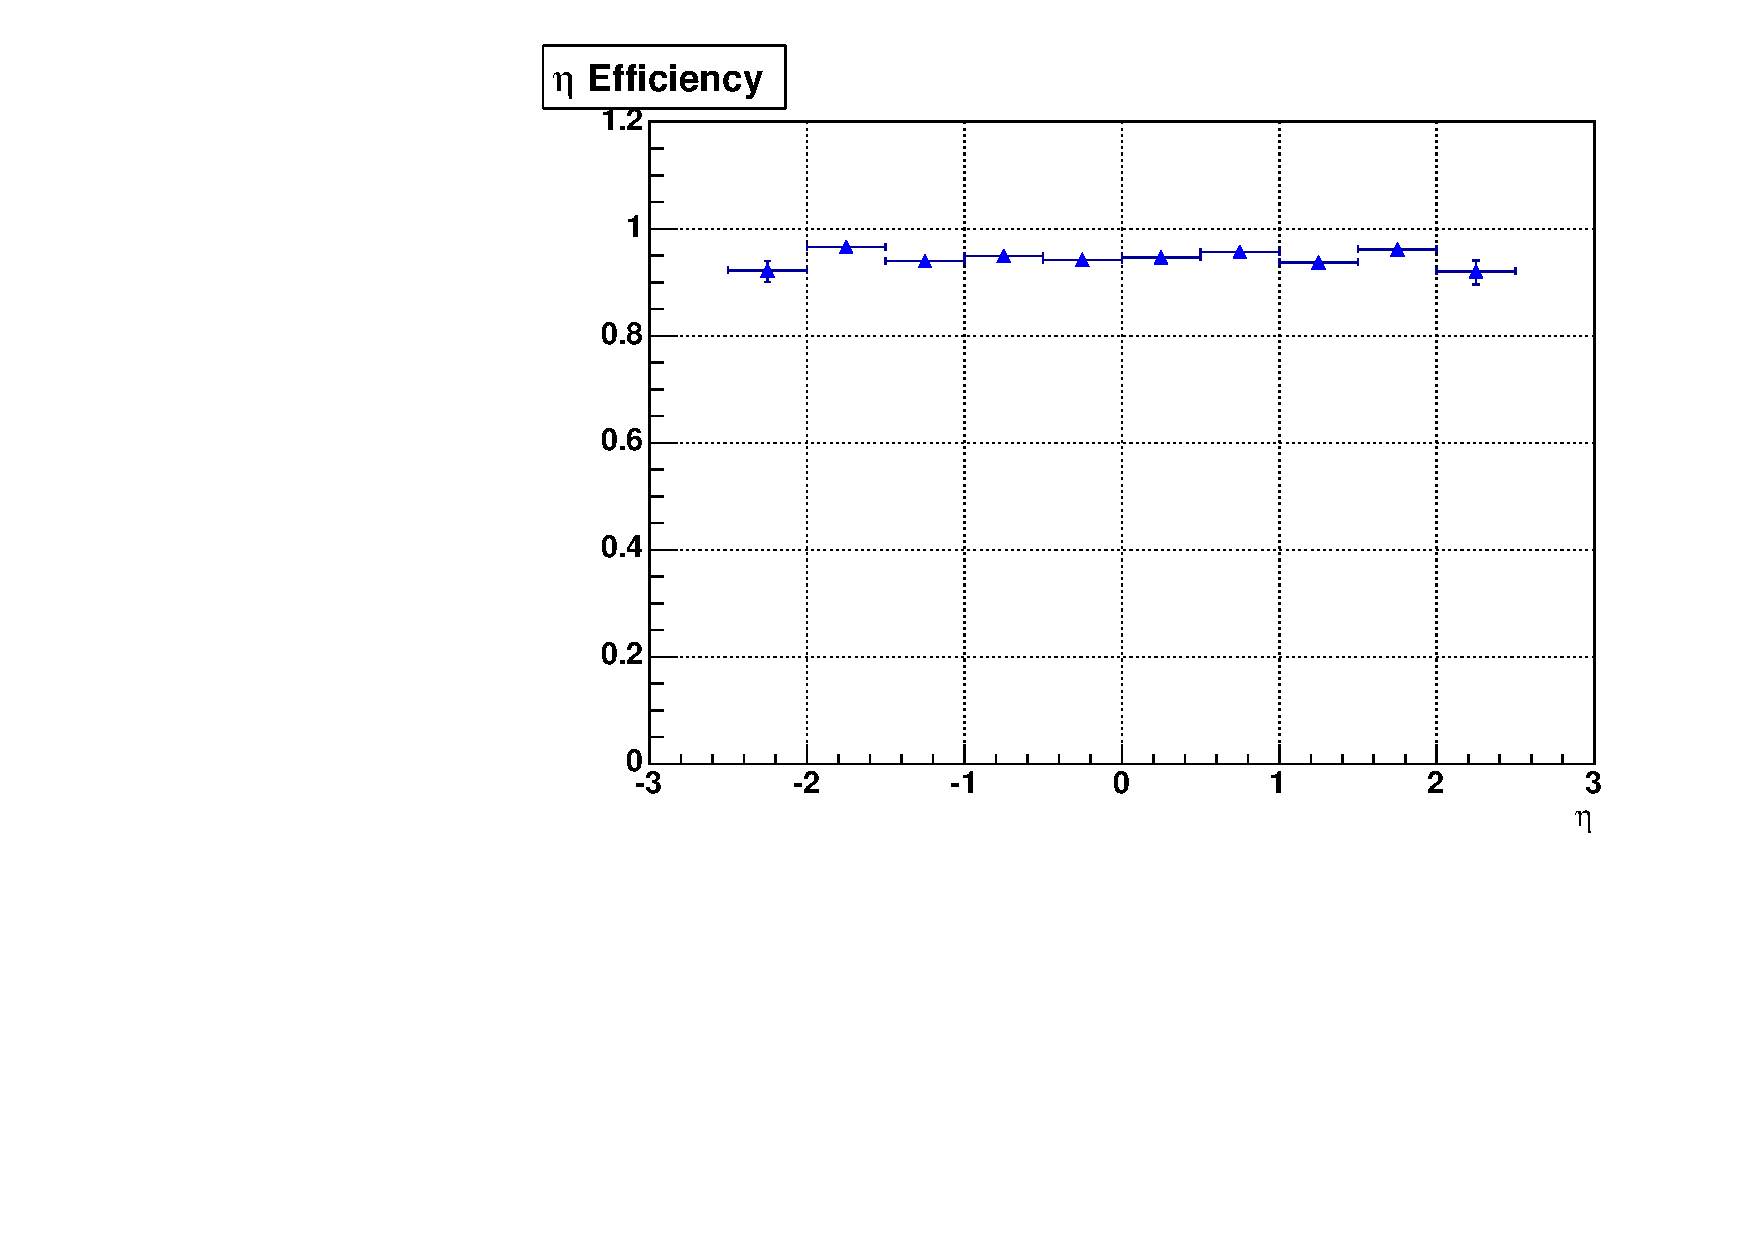
\includegraphics[width=\cmsFigWidth]{figures/soft_eta_eff}
    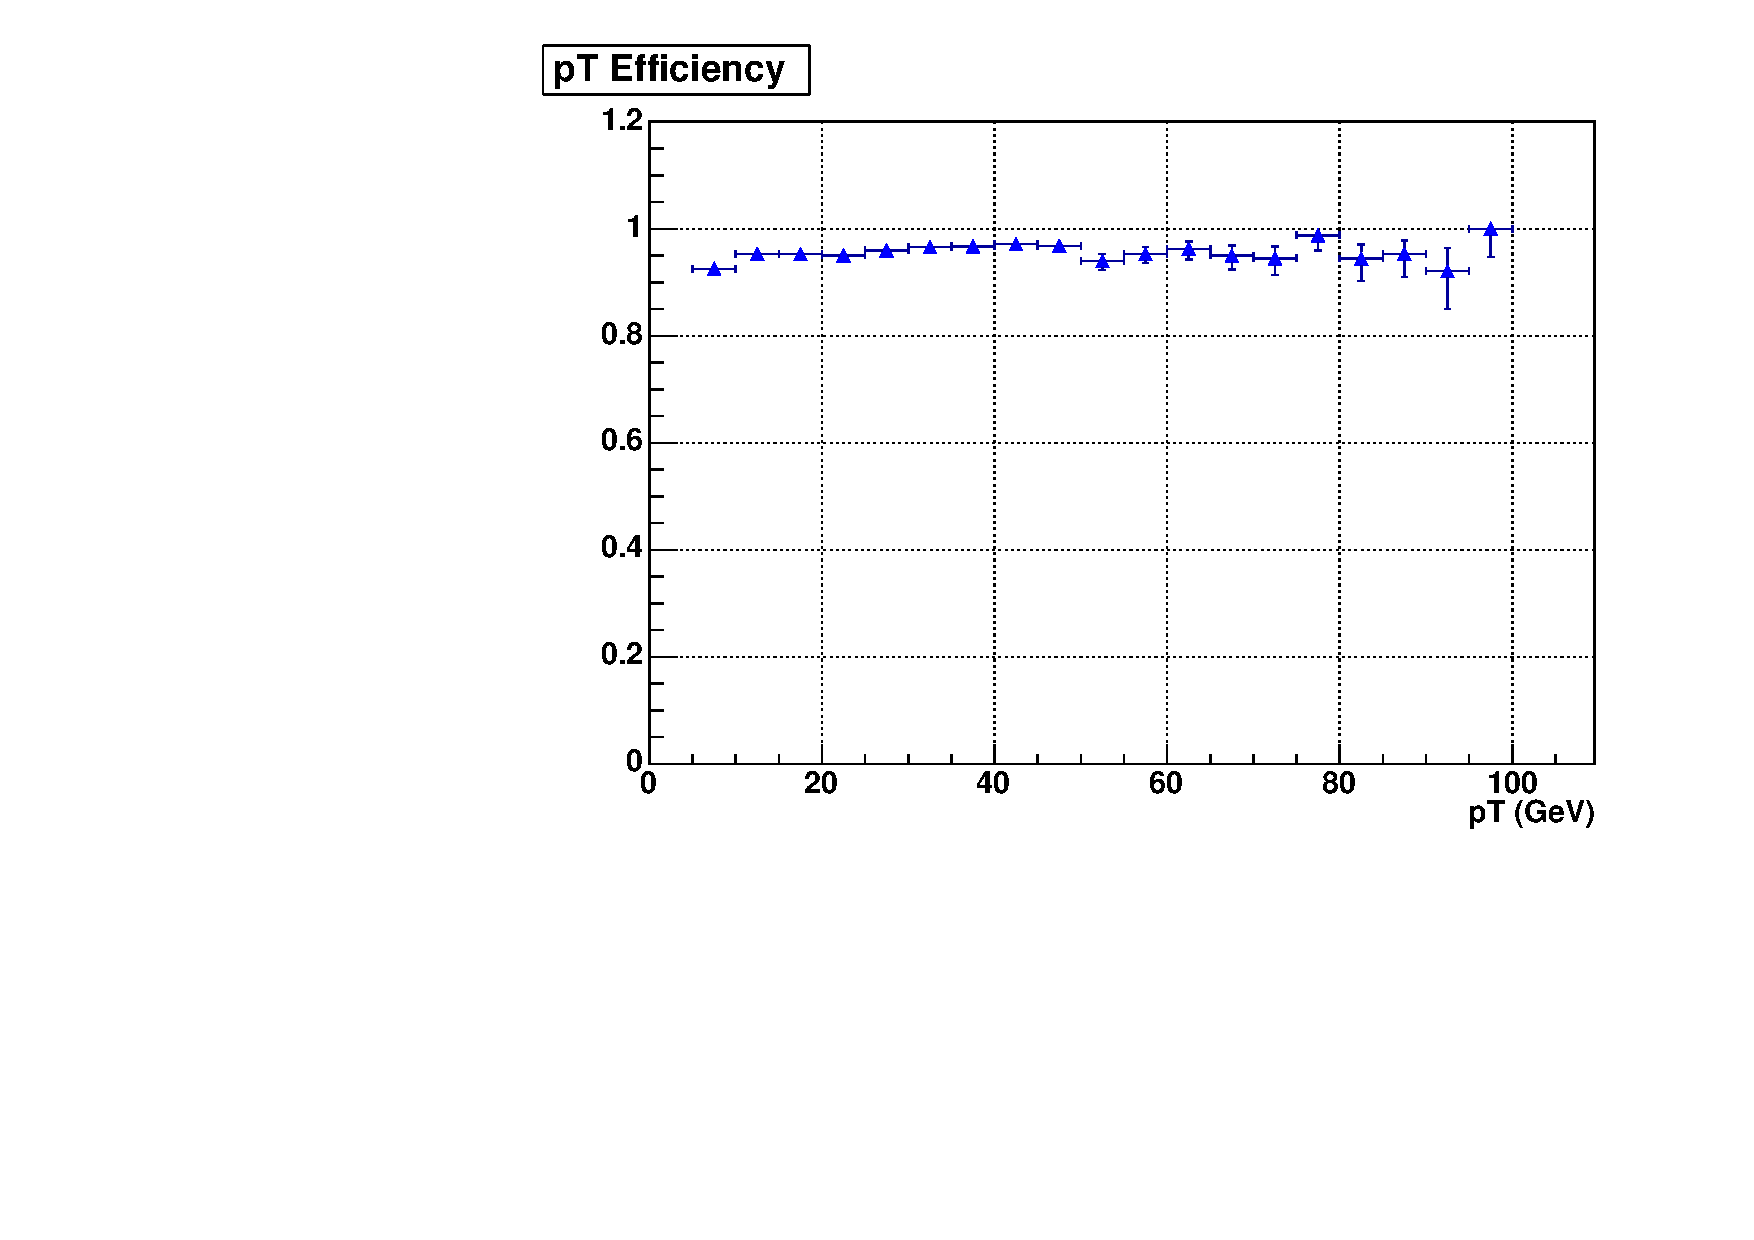
\includegraphics[width=\cmsFigWidth]{figures/soft_pt_eff}
    \caption{Soft muon efficiency as a function of $\eta$ (\cmsLeft) and $p_T$ (\cmsRight) in WH signal events. Errors are statistical only.}
    \label{fig:soft_muon}
  \end{center}
\end{figure}

The WH soft muon efficiency is $\sim$95\% across a range of $\eta$ and $p_T$ and is in good qualitative agreement with soft muon efficiencies measured in CMS data $J\slash\psi\rightarrow\mu\mu$ events~\cite{1748-0221-7-10-P10002}.  As the MUO POG measured soft muon efficiency agrees with the value from $J\slash\psi\rightarrow\mu\mu$ simulation~\cite{CMS:muonrefeffstwiki} within the quoted error, the signal WH and ggH MC is not corrected for differences from data.  Instead, the MUO POG recommended error of 1.5\% is propagated to the error on the expected signal.

%HPS tau id efficiency (Minsoo)
\subsection{HPS tau\label{sec:HPS-id}}

The MC sample \texttt{/DYJetsToLL\_M-50\_TuneZ2star\_8TeV-madgraph-tarball/\\Summer12\_DR53X-PU\_S10\_START53\_V7A-v1/AODSIM} is used to calculate HPS tau efficiency on $Z\rightarrow\tau_{\mu}\tau_{\text{had}}$ events.  The $\tau_{\mu}$ leg of the $Z$ decay is required to fire \texttt{HLT\_IsoMu24\_eta2p1} and pass the trigger muon ID.  HPS decay mode finding and isolation efficiency are measured on the $\tau_{\text{had}}$ leg.  For WH signal events, in addition to the trigger muon ID described above, the HPS tau is required to be built from a jet cleaned of a soft muon (cf. Sec.~\ref{sec:evtsel-ditau}).

The $p_T$ distributions of gen-level taus matched to reconstructed HPS taus are shown in Figure~\ref{fig:gen_whtt} for the WH sample and Figure~\ref{fig:gen_ztt} for the $Z\rightarrow\tau\tau$ sample.  Gen-matching is performed in a cone of $\Delta$R = 0.3 around the reconstructed HPS tau.  Signal WH taus tend to be softer than $Z$ decay taus, yet their ID and isolation efficiencies are similar as shown below.

\begin{figure}[hbtp]
  \begin{center}
    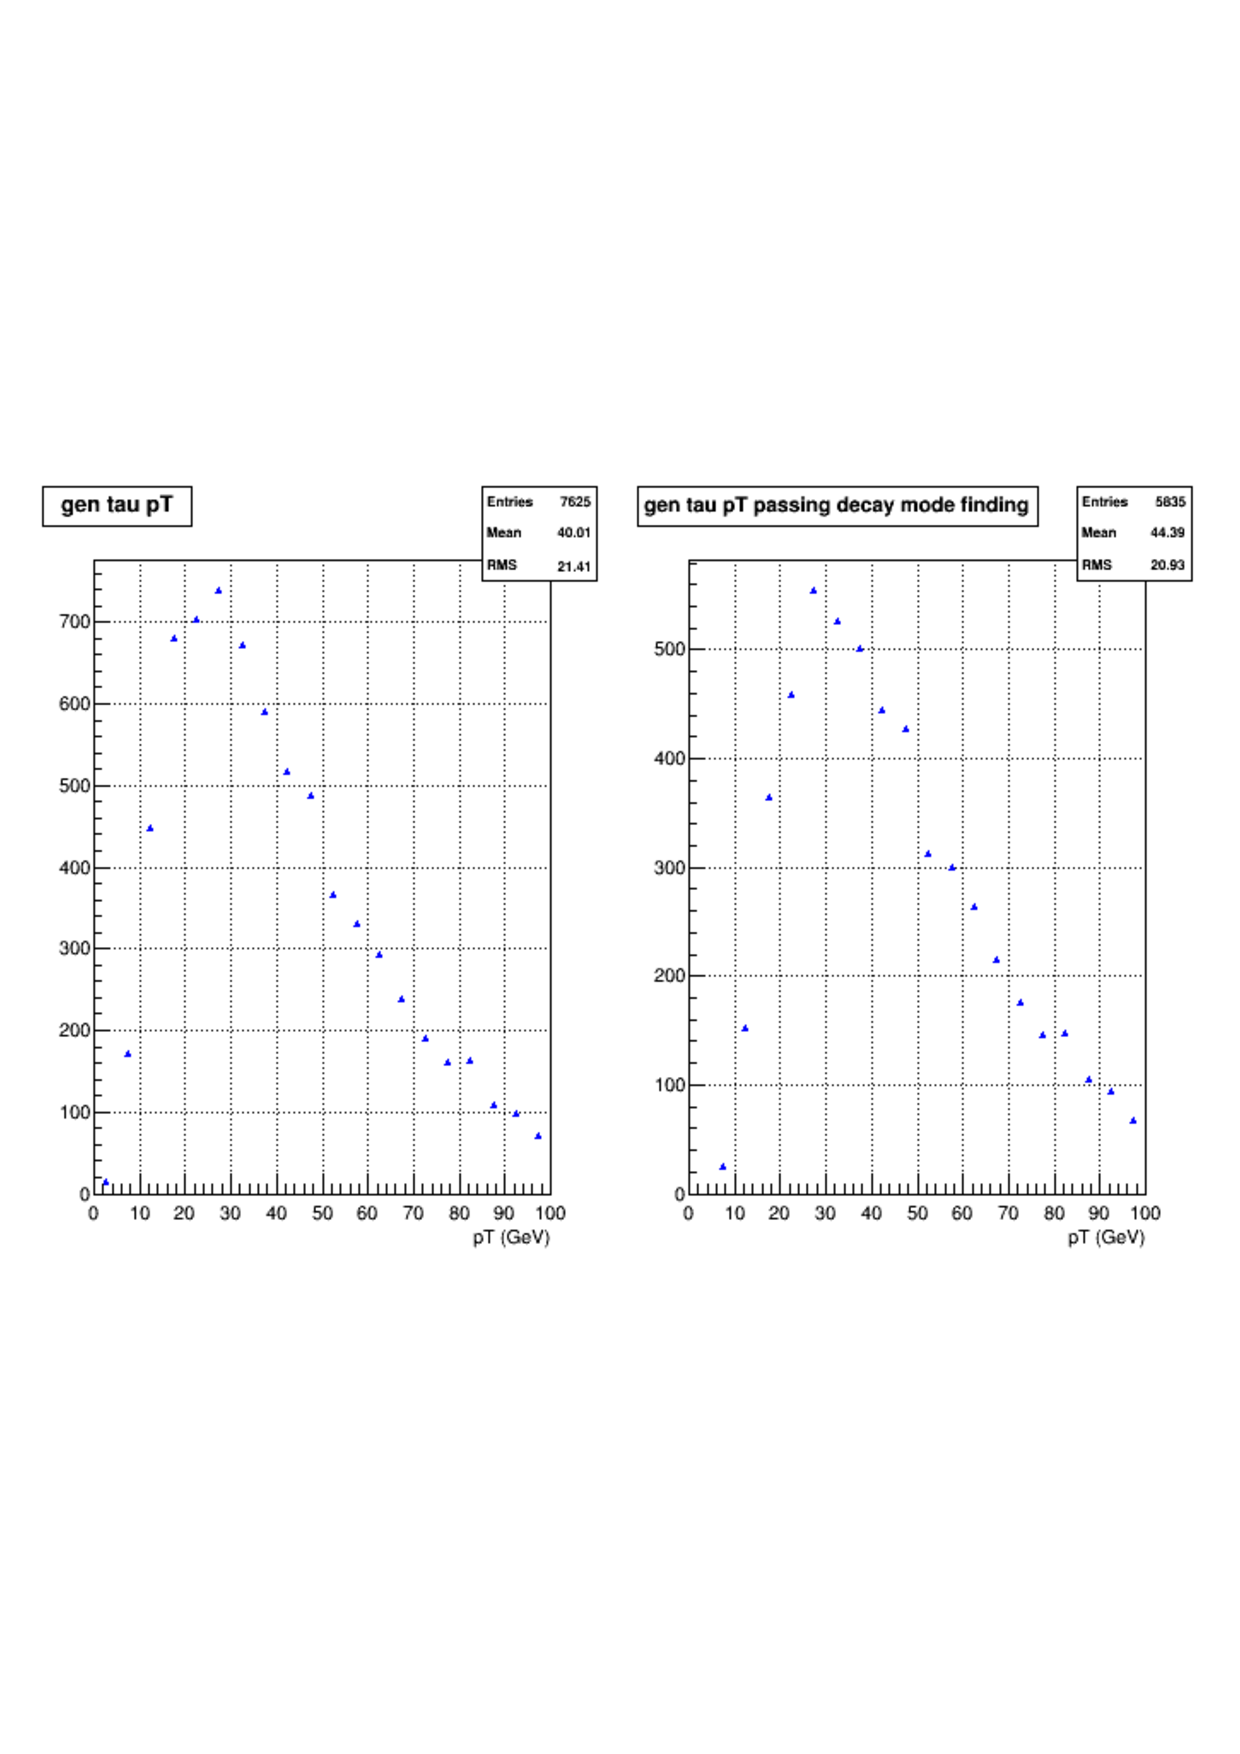
\includegraphics[width=\cmsFigWidth]{figures/pT_whtt_DMF}
    \caption{$p_T$ of gen taus from WH $\tau_{\mu}\tau_{\text{had}}$ pairs matched to reconstructed HPS taus with associated soft muons (cf. Sec.~\ref{sec:evtsel-ditau}).  Errors are statistical only.  (\cmsLeft) No discriminator requirement.  (\cmsRight) \texttt{DecayModeFinding} requirement.}
    \label{fig:gen_whtt}
  \end{center}
\end{figure}

\begin{figure}[hbtp]
  \begin{center}
    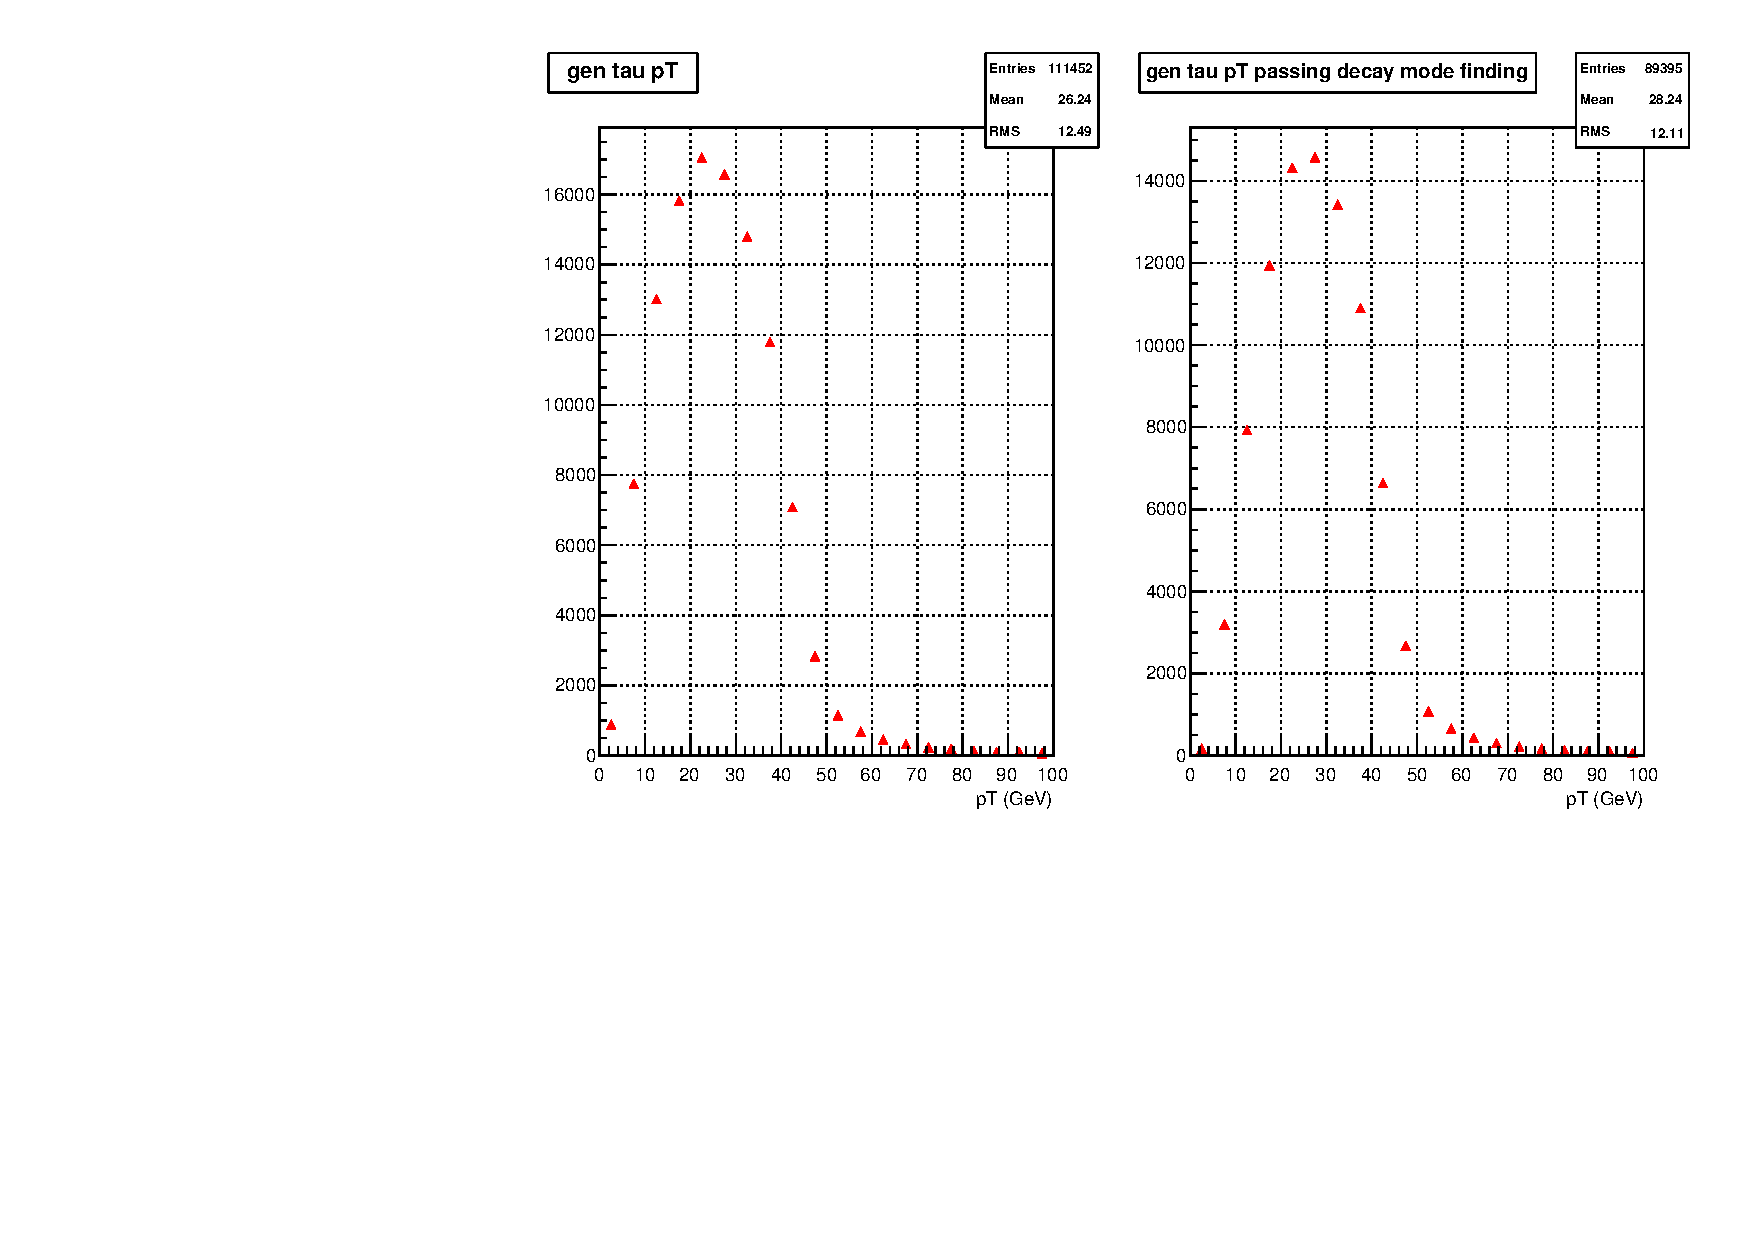
\includegraphics[width=\cmsFigWidth]{figures/gentau_pt_ztt_dmf}
    \caption{$p_T$ of gen taus from $Z\rightarrow\tau\tau$ decay matched to standard reconstructed HPS taus.  Errors are statistical only.  (\cmsLeft) No discriminator requirement.  (\cmsRight) \texttt{DecayModeFinding} requirement.}
    \label{fig:gen_ztt}
  \end{center}
\end{figure}

The decay mode finding efficiency $\epsilon_{\text{DMF}}$ = (number of gen-matched HPS taus in $\abs{\eta} <$ 2.4 passing the \texttt{DecayModeFinding} discriminator)/(number of gen-matched HPS taus in \abs{\eta} \textless\xspace 2.4) is shown for WHand $Z\rightarrow\tau\tau$ events in Figure~\ref{fig:eff_dmf} (\cmsLeft).  There is good agreement across a range of $\eta$ and $p_T$ between the simulated efficiency for signal boosted tau pair events reconstructed with the cleaning procedure described in Sec.~\ref{sec:evtsel-tauID} and $Z\rightarrow\tau_{\mu}\tau_{\text{had}}$ events.  In particular, the agreement is good even for relatively low tau $p_T$ ($<$ 20 GeV).  Similarly, the decay mode finding and isolation efficiency $\epsilon_{\text{DMF+iso}}$ = (number of gen-matched HPS taus in $\abs{\eta} <$ 2.4 passing the \texttt{DecayModeFinding} and \texttt{MediumCombinedIsolationDBSumPtCorr} discriminators)/(number of gen-matched HPS taus in $\abs{\eta} <$ 2.4) is shown in Figure~\ref{fig:eff_dmf_mi}. There is qualitative agreement with public TAU POG efficiencies for simulated $Z\rightarrow\tau\tau$ events~\cite{CMS:approvedTAUResults}.

\begin{figure}[hbtp]
  \begin{center}
    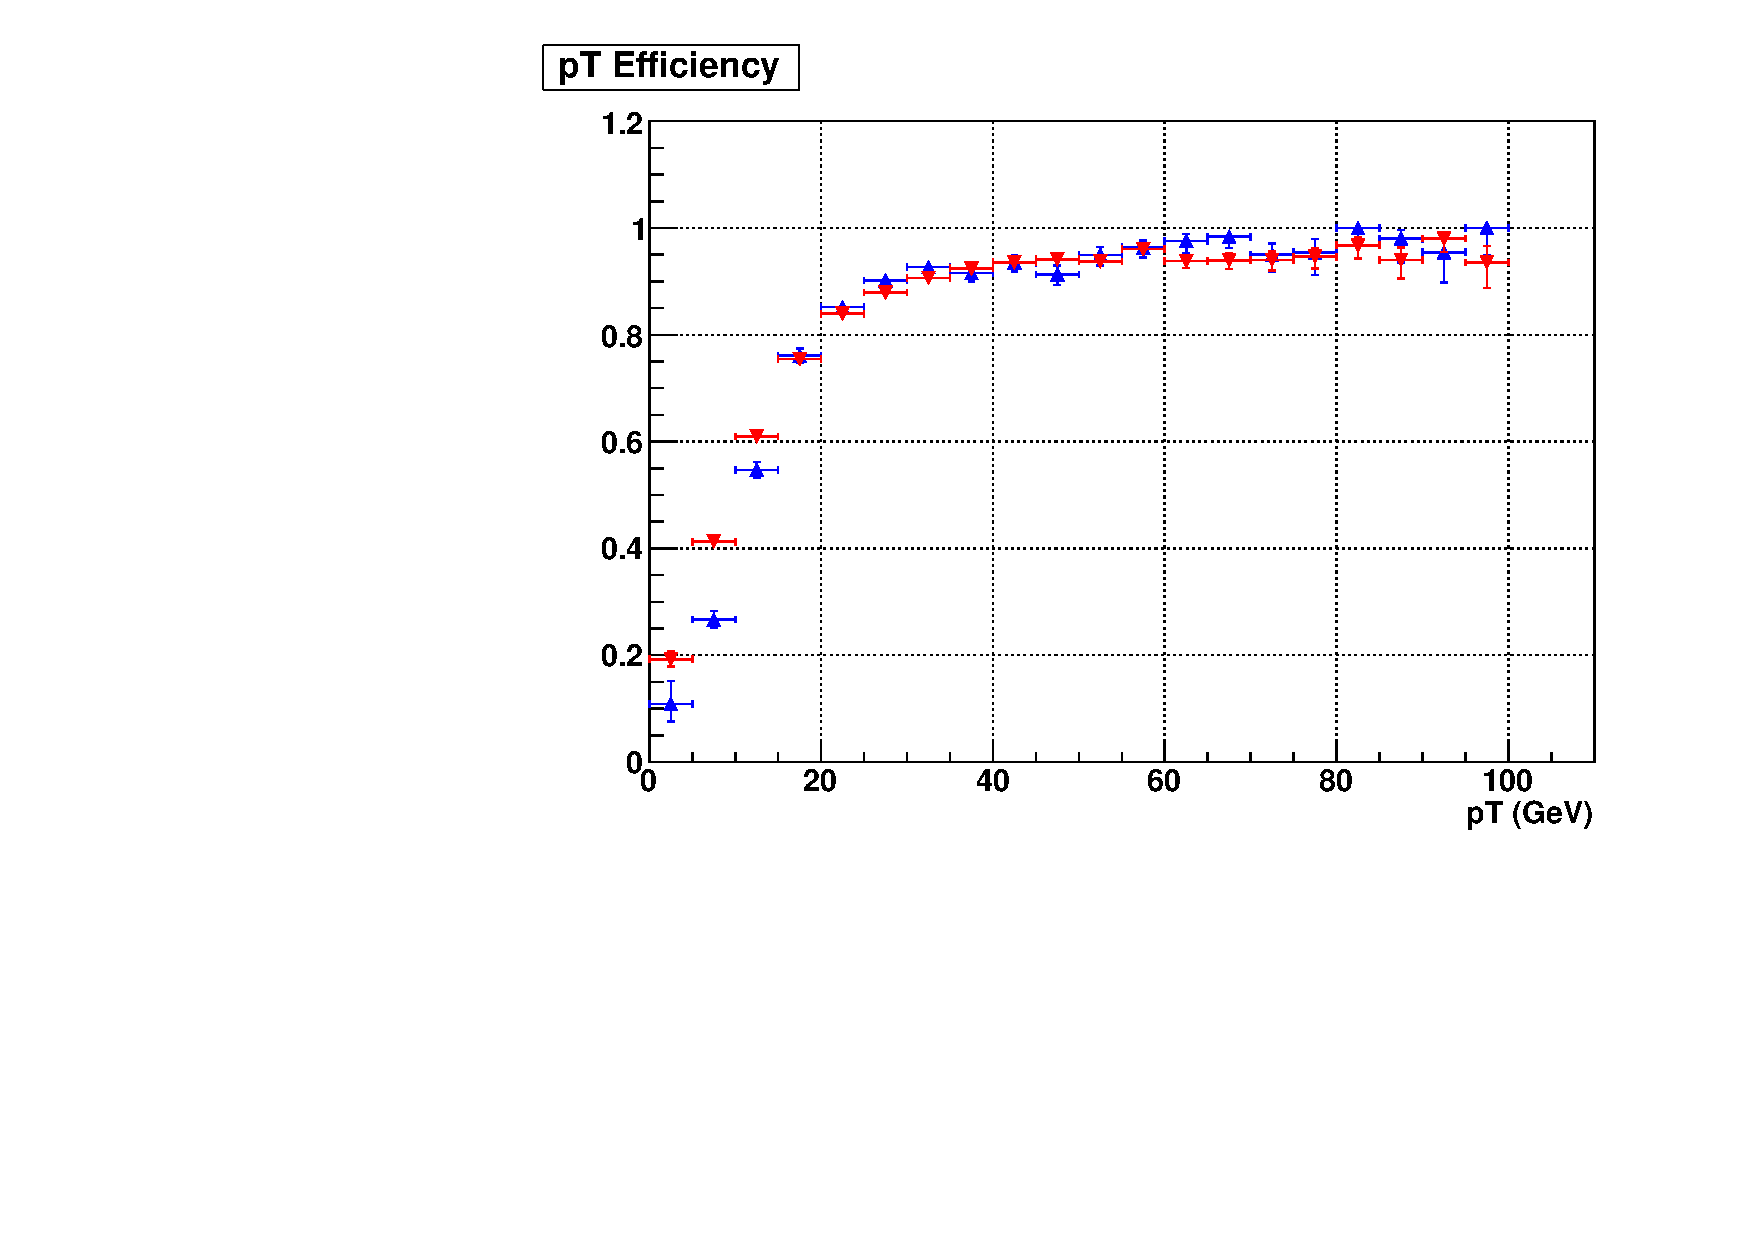
\includegraphics[width=\cmsFigWidth]{figures/gentau_dmf_pt}
    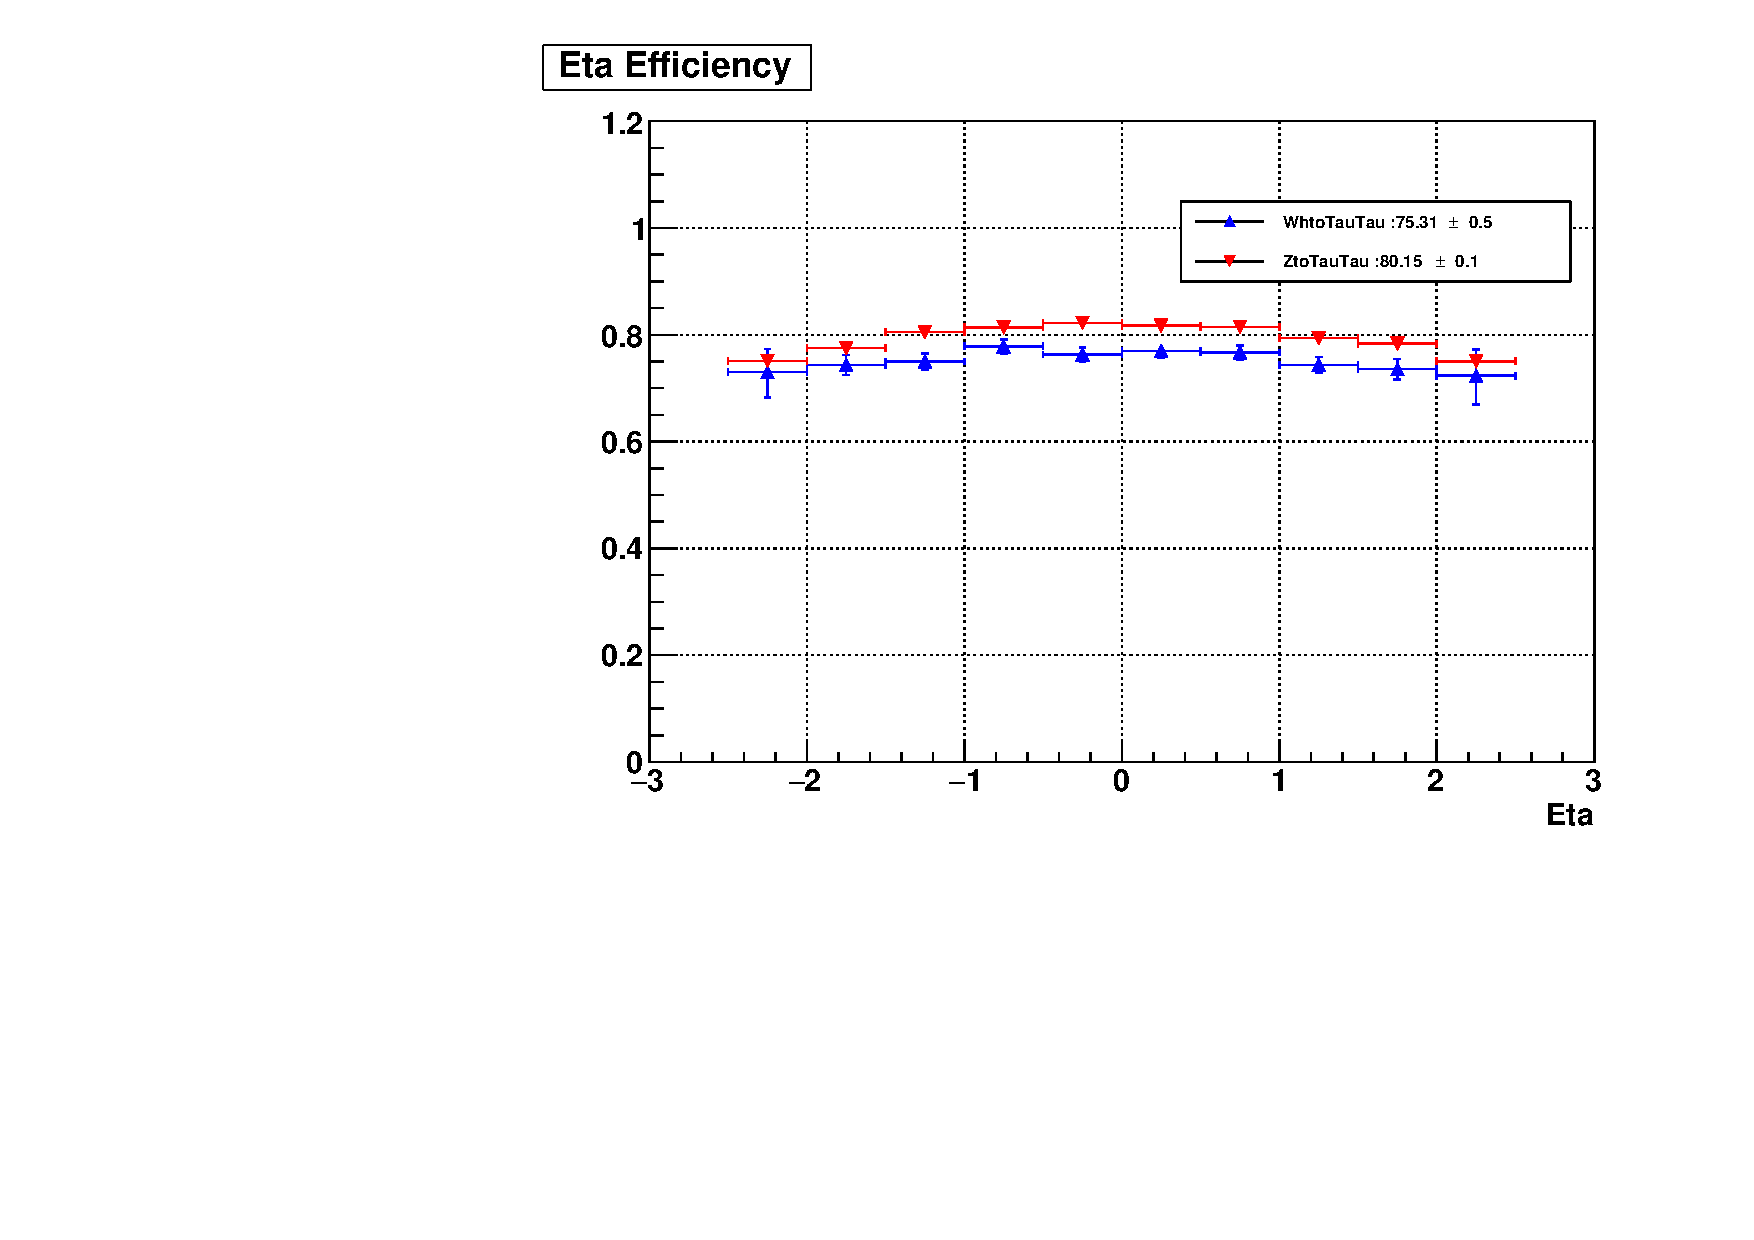
\includegraphics[width=\cmsFigWidth]{figures/gentau_dmf_eta}
    \caption{(\cmsLeft) HPS decay mode finding efficiency as a function of matched gen tau $p_T$. (\cmsRight) HPS decay mode finding efficiency as a function of matched gen tau $\eta$.  Signal HPS taus (blue) are reconstructed using the soft muon cleaning procedure described in this document, while taus from $Z$ decay (red) are reconstructed with standard HPS. Errors are statistical only.}
    \label{fig:eff_dmf}
  \end{center}
\end{figure}

\begin{figure}[hbtp]
  \begin{center}
    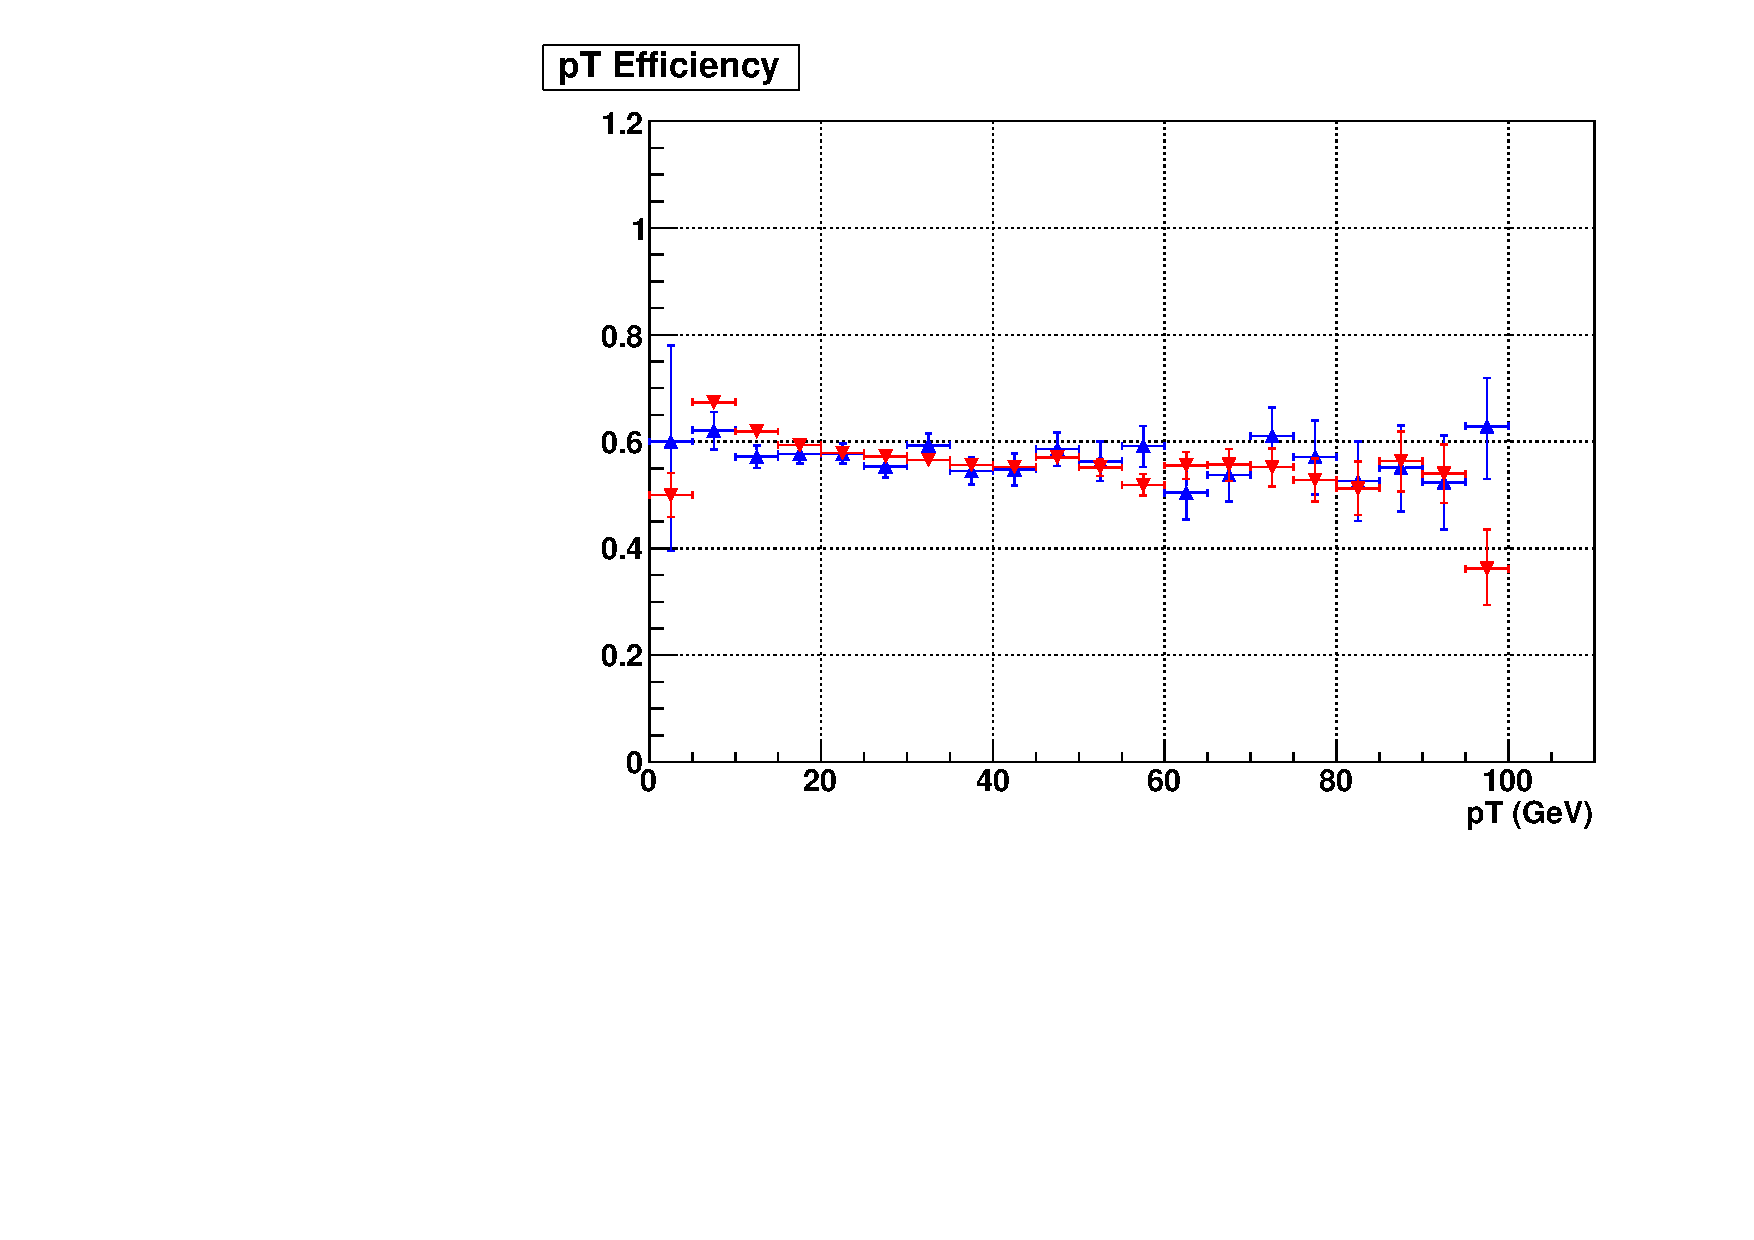
\includegraphics[width=\cmsFigWidth]{figures/gentau_dmfmi_pt}
    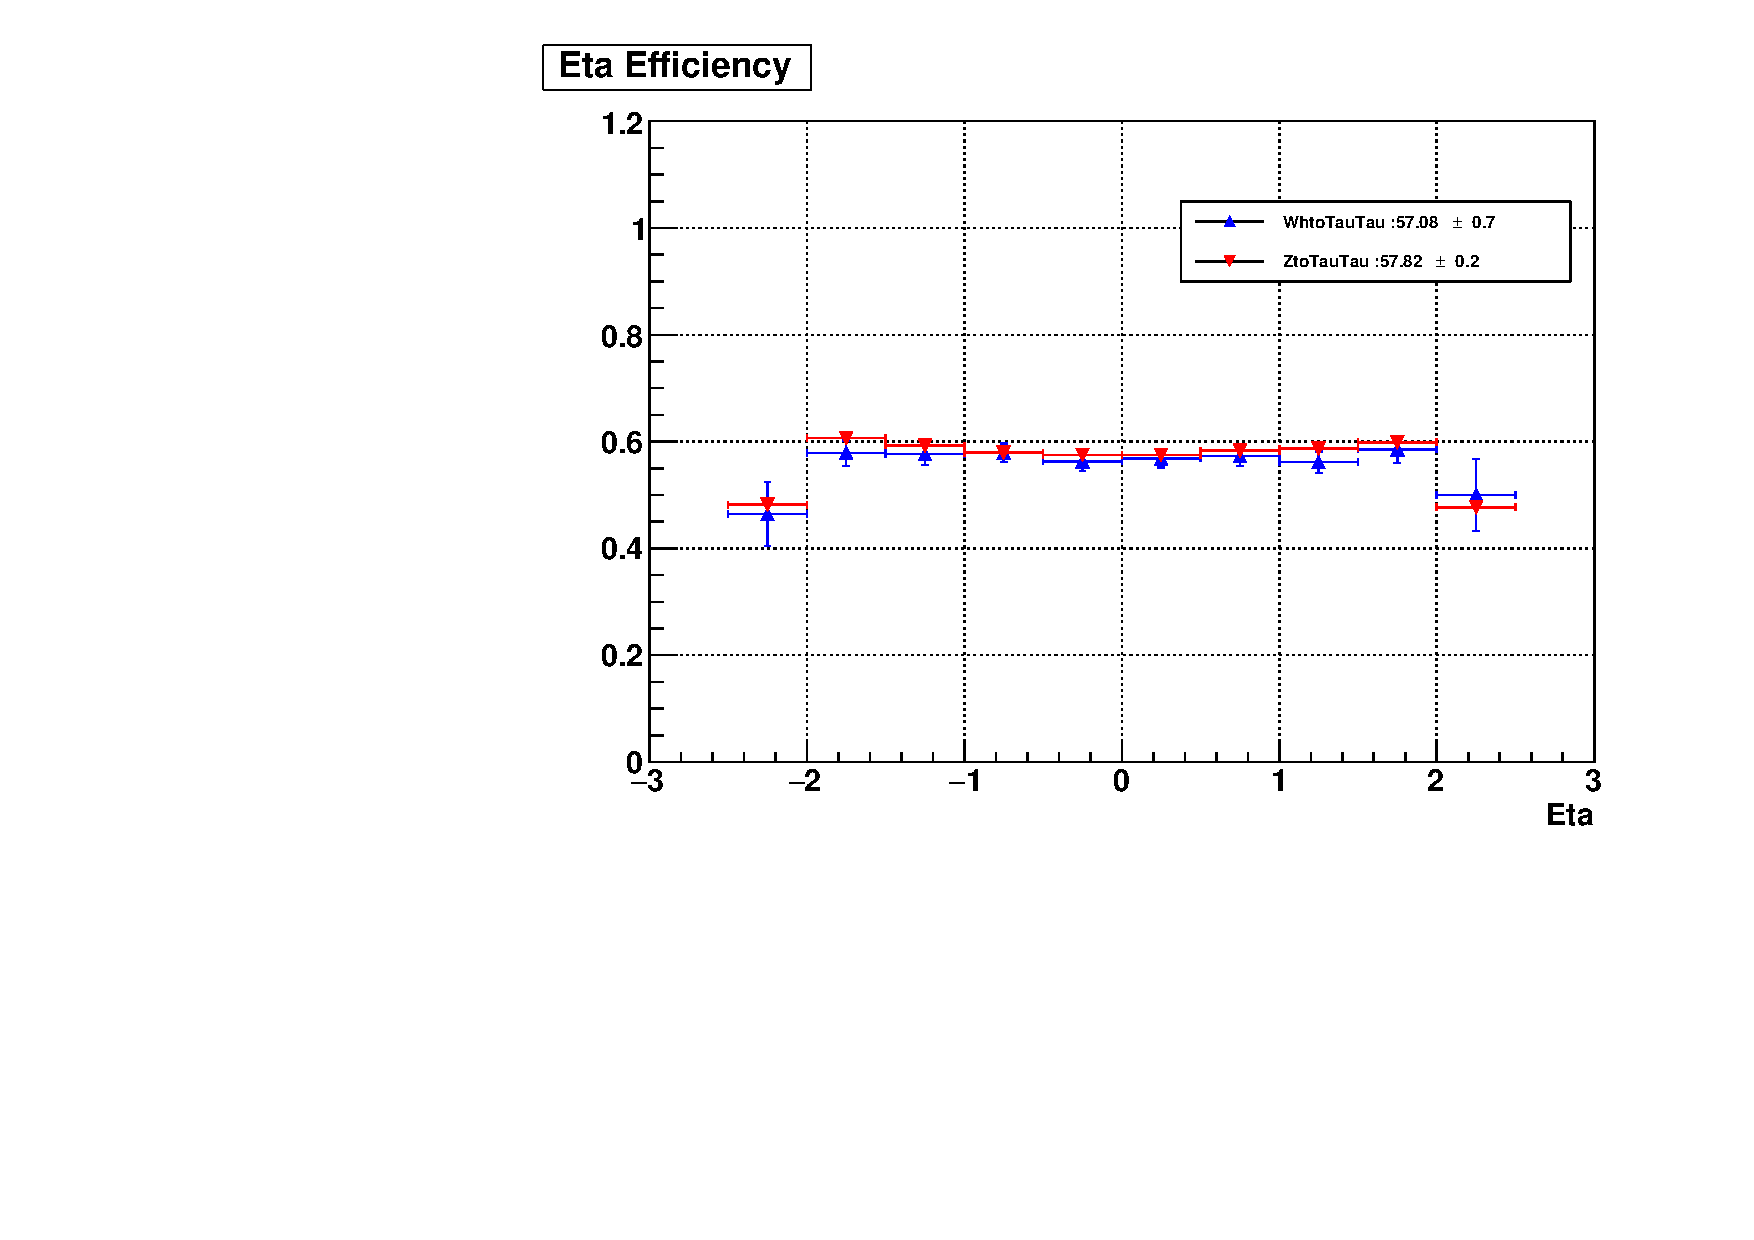
\includegraphics[width=\cmsFigWidth]{figures/gentau_dmfmi_eta}
    \caption{(\cmsLeft) HPS decay mode finding + medium combined isolation efficiency as a function of matched gen tau $p_T$. (\cmsRight) HPS decay mode finding efficiency as a function of matched gen tau $\eta$.  Signal HPS taus (blue) are reconstructed using the soft muon cleaning procedure described in this document, while taus from $Z$ decay (red) are reconstructed with standard HPS. Errors are statistical only.}
    \label{fig:eff_dmf_mi}
  \end{center}
\end{figure}

%As in the case of the soft muon, differences in the TAU POG approved HPS decay mode finding and isolation efficiencies between data and MC are within errors~\cite{CMS:tauuncertaintytwiki}, so instead of correcting the signal MC we simply propagate the recommended error of 6\% to the expected signal.
To cover discrepancies of up to about 10\% between the efficiencies in the signal and in $Z\rightarrow\tau_{\mu}\tau_{\text{had}}$, the TAU POG has recommended a conservative systematic of 10\% to apply to the HPS tau ID efficiency data-MC scale factor when a $p_T$ cut of 10 GeV is used. The $p_T$ cut used for the $\tau_{\text{had}}$ from the $\tau_{\mu}\tau_{\text{had}}$ object is 20 GeV; however, this efficiency study is still important because a $p_T$ cut of 10 GeV is applied to taus in the neighbouring lepton veto for the trigger muon (in order to have a better efficiency for the veto), and because future iterations of this search may explore the possibility of lowering the $p_T$ cut on the $\tau_{\text{had}}$ from $\tau_{\mu}\tau_{\text{had}}$ as well, as was originally intended.

Since the HPS tau ID efficiencies and scale factors have been validated by the TAU POG only down to 20 GeV, a study was done to reconstruct the \Z peak using HPS taus with $p_T$ between 10 and 20 GeV and to compare it to the $Z$ peak reconstructed from HPS taus with $p_T >$ 20 GeV, to assess the reliability of using taus with $p_T$ between 10 and 20 GeV. $Z\rightarrow\tau_{\mu}\tau_{\text{had}}$ events were selected in the MC sample \texttt{/DYJetsToLL\_M-50\_TuneZ2star\_8TeV-madgraph-tarball/\\Summer12\_DR53X-PU\_S10\_START53\_V7A-v1/AODSIM}; the $\tau_{\mu}$ leg of the \Z decay wass required to fire \texttt{HLT\_IsoMu24\_eta2p1}, pass the trigger muon ID, and be gen-matched to the $Z$ decay, while the gen-matched HPS tau was required to pass \texttt{DecayModeFinding} and \texttt{MediumCombined\\IsolationDBSumPtCorr} discriminators and a $p_T$ cut of either $>$ 20 GeV for the standard case, or between 10 and 20 GeV for the low-$p_T$ case of interest. As shown in Figure~\ref{fig:Zpeakstudy}, the Z peak looks normal for HPS tau $p_T$ \textgreater\xspace 20 GeV, and the Z peak shape for the low-$p_T$ range looks normal aside from being biased to a lower mean due to the lower HPS tau $p_T$ cut.

\begin{figure}[hbtp]
  \begin{center}
    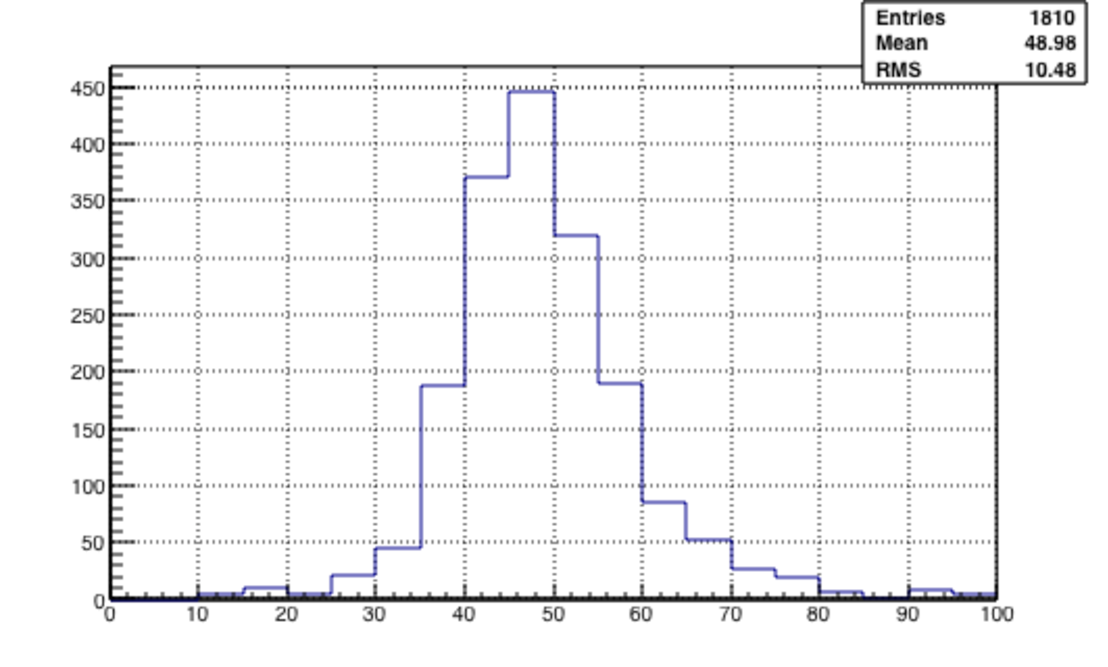
\includegraphics[width=\cmsFigWidth]{figures/gen_muhad_mass_1020}
    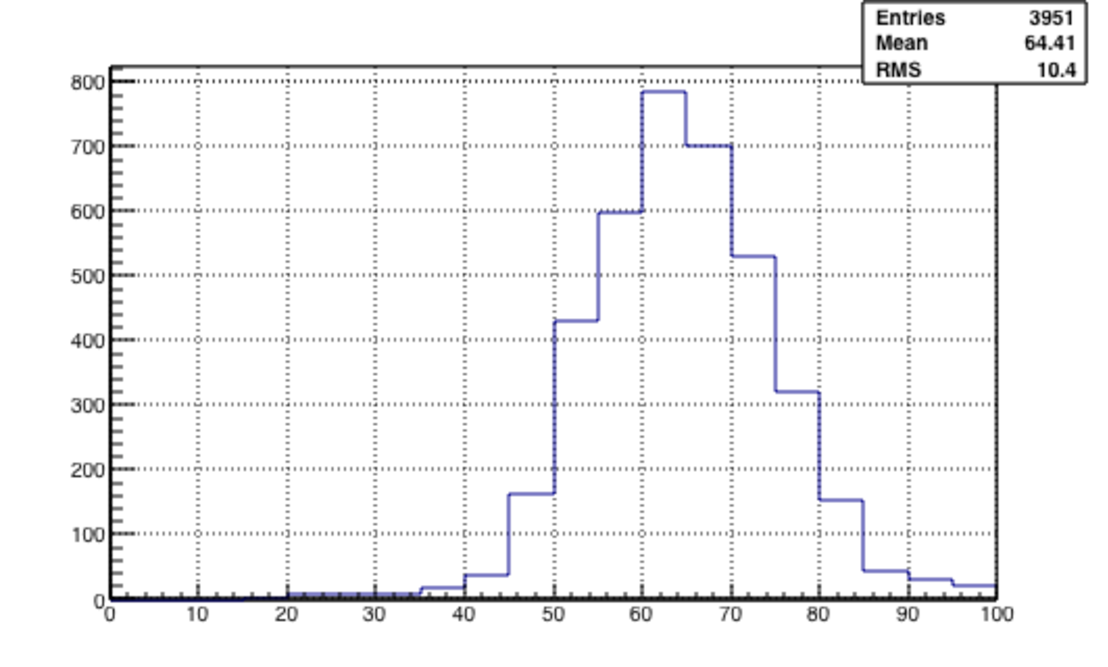
\includegraphics[width=\cmsFigWidth]{figures/gen_muhad_mass_20}
    \caption{Z peak reconstructed in a sample of Drell-Yan MC events. (\cmsLeft) HPS tau $p_T$ between 10 and 20 GeV. (\cmsRight) HPS tau $p_T <$ 20 GeV.}
    \label{fig:Zpeakstudy}
  \end{center}
\end{figure}